\pdfoutput=1
\documentclass{article}

% if you need to pass options to natbib, use, e.g.:
\PassOptionsToPackage{numbers, compress}{natbib}
% before loading neurips_2023

% to compile a camera-ready version, add the [final] option, e.g.:
\usepackage[final,nonatbib]{neurips_2023}
    

\usepackage[utf8]{inputenc} % allow utf-8 input
\usepackage[T1]{fontenc}    % use 8-bit T1 fonts
\usepackage{hyperref}       % hyperlinks
\usepackage{url}            % simple URL typesetting
\usepackage{booktabs}       % professional-quality tables
\usepackage{amsfonts}       % blackboard math symbols
\usepackage{nicefrac}       % compact symbols for 1/2, etc.
\usepackage{microtype}      % microtypography
\usepackage{xcolor}         % colors



% math commands
%%%%% NEW MATH DEFINITIONS %%%%%
\usepackage{amsmath}
\usepackage{amsfonts} 
\usepackage{bm}

\def\vzero{{\bm{0}}}
\def\vone{{\bm{1}}}
\def\vmu{{\bm{\mu}}}
\def\vtheta{{\bm{\theta}}}
\def\vomega{{\bm{\omega}}}
\def\veta{{\bm{\eta}}}
\def\vtau{{\bm{\tau}}}
\def\vphi{{\bm{\phi}}}
\def\vpsi{{\bm{\psi}}}
\def\rvepsilon{{\mathbf{\epsilon}}}
\def\rvtheta{{\mathbf{\theta}}}
\def\rvphi{{\mathbf{\phi}}}
\def\rveta{{\mathbf{\eta}}}
\newcommand{\E}{\mathbb{E}}
\newcommand{\KL}{D_{\mathrm{KL}}}
\DeclareMathOperator*{\argmax}{arg\,max}
\DeclareMathOperator*{\argmin}{arg\,min}
\newcommand{\oa}{\obs, \act}
\newcommand{\oan}{\obs_n, \act_n}
\newcommand{\exz}{\E_{p(z)}}
\newcommand{\cur}{p(\obs, \act)}
\newcommand{\curpc}{p(\obs, \act|z)}
\newcommand{\entcur}{\mathcal{H}(\obs, \act)}
\newcommand{\entcurpc}{\mathcal{H}(\obs, \act|z)}
\newcommand{\optcur}{p^*(\obs, \act)}
\newcommand{\optcurpc}{p^*(\obs, \act|z)}
\newcommand{\curn}{p(\obs_n, \act_n)}
\newcommand{\curnpz}{p(\obs_n, \act_n|z)}
\newcommand{\optcurn}{p^*(\obs_n, \act_n)}
\newcommand{\excur}{\E_{\cur}}
\newcommand{\excurpc}{\E_{\curpc}}
\newcommand{\expert}{\log p_{\vtheta}(\act|\obs)}
\newcommand{\expertn}{\log p_{\vtheta}(\act_n|\obs_n)}
\newcommand{\expertpc}{\log p_{\vtheta_\comp}(\act|\obs,z)}
\newcommand{\expertnpc}{\log p_{\vtheta_\comp}(\act_n|\obs_n, z)}
\newcommand{\obs}{\mathbf{o}}
\newcommand{\act}{\mathbf{a}}
\newcommand{\comp}{z}

% Recommended, but optional, packages for figures and better typesetting:
\usepackage{microtype}
% \usepackage{graphicx}
%\usepackage{subfigure}
\usepackage{subcaption}
\usepackage{booktabs} % for professional tables


% If accepted, instead use the following line for the camera-ready submission:
% \usepackage{neurips_2023}

% For theorems and such
\usepackage{amsmath}
\usepackage{amssymb}
\usepackage{mathtools}
\usepackage{amsthm}

% Use fancyhdr package
\RequirePackage{fancyhdr}
\RequirePackage{xcolor} % changed from color to xcolor (2021/11/24)
\RequirePackage{algorithm}
\RequirePackage{algorithmic}
\RequirePackage{natbib}
\RequirePackage{eso-pic} % used by \AddToShipoutPicture
\RequirePackage{forloop}
\RequirePackage{url}

\usepackage{graphicx,lipsum,wrapfig}

% if you use cleveref..
\usepackage[capitalize,noabbrev]{cleveref}

% \input{mathcommands.tex}


% \theoremstyle{proposition}
\newtheorem{proposition}{Proposition}[section]
% \theoremstyle{corollary}
% \newtheorem{corollary}{Corollary}[proposition]

\newtheorem{corollaryinner}{Corollary}[proposition] % just the internal version
\newenvironment{corollary}[1][]
 {% #1 is the cross reference label
  \if\relax\detokenize{#1}\relax
    % we have a corollary directly following a theorem, do nothing special
  \else
    \ifcsname #1-used\endcsname
      \expandafter\xdef\csname #1-used\endcsname{\the\numexpr\csname #1-used\endcsname+1}%
    \else
      \expandafter\gdef\csname #1-used\endcsname{1}%
    \fi
    \renewcommand{\thecorollaryinner}{\ref{#1}.\csname #1-used\endcsname}%
  \fi
  \corollaryinner
 }
 {\endcorollaryinner}


\title{Information Maximizing Curriculum: \\ \Large{A Curriculum-Based Approach for Imitating Diverse Skills}}


% The \author macro works with any number of authors. There are two commands
% used to separate the names and addresses of multiple authors: \And and \AND.
%
% Using \And between authors leaves it to LaTeX to determine where to break the
% lines. Using \AND forces a line break at that point. So, if LaTeX puts 3 of 4
% authors names on the first line, and the last on the second line, try using
% \AND instead of \And before the third author name.


\author{%
  Denis Blessing
  \thanks{Correspondence to \texttt{denis.blessing@kit.edu}}$\textcolor{white}{i}^\dagger$
     Onur Celik$^{\dagger \S}$ Xiaogang Jia$^{\dagger \ddagger}$ Moritz Reuss$^{\ddagger}$ 
    \\ 
    \textbf{Maximilian Xiling Li$^{\ddagger}$  Rudolf Lioutikov$^{\ddagger}$  Gerhard Neumann$^{\dagger \S}$} 
    \\
  $^{\dagger}$ Autonomous Learning Robots, Karlsruhe Institute of Technology \\
  $^{\ddagger}$ Intuitive Robots Lab, Karlsruhe Institute of Technology \\
  $^{\S}$ FZI Research Center for Information Technology 
  % \\
  % Pittsburgh, PA 15213 \\
  % \texttt{hippo@cs.cranberry-lemon.edu
  % } \\
  % examples of more authors
  % \And
  % Coauthor \\
  % Affiliation \\
  % Address \\
  % \texttt{email} \\
  % \AND
  % Coauthor \\
  % Affiliation \\
  % Address \\
  % \texttt{email} \\
  % \And
  % Coauthor \\
  % Affiliation \\
  % Address \\
  % \texttt{email} \\
  % \And
  % Coauthor \\
  % Affiliation \\
  % Address \\
  % \texttt{email} \\
}


\begin{document}


\maketitle



Over the past few years, there has been a significant amount of research focused on studying the ReLU activation function, with the aim of achieving neural network convergence through over-parametrization. However, recent developments in the field of Large Language Models (LLMs) have sparked interest in the use of exponential activation functions, specifically in the attention mechanism.

Mathematically, we define the neural function $F: \R^{d \times m} \times  \mathbb{R}^d \rightarrow \mathbb{R}$ using an exponential activation function. Given a set of data points with labels $\{(x_1, y_1), (x_2, y_2), \dots, (x_n, y_n)\} \subset \mathbb{R}^d \times \mathbb{R}$ where $n$ denotes the number of the data. Here $F(W(t),x)$ can be expressed as $F(W(t),x) := \sum_{r=1}^m a_r \exp(\langle w_r, x \rangle)$, where $m$ represents the number of neurons, and $w_r(t)$ are weights at time $t$. It's standard in literature that $a_r$ are the fixed weights and it's never changed during the training. We initialize the weights $W(0) \in \mathbb{R}^{d \times m}$ with random Gaussian distributions, such that $w_r(0) \sim \mathcal{N}(0, I_d)$ and initialize $a_r$ from random sign distribution for each $r \in [m]$.

Using the gradient descent algorithm, we can find a weight $W(T)$ such that $\| F(W(T), X) - y \|_2 \leq \epsilon$ holds with probability $1-\delta$, where $\epsilon \in (0,0.1)$ and $m = \Omega(n^{2+o(1)}\log(n/\delta))$. To optimize the over-parametrization bound $m$, we employ several tight analysis techniques from previous studies [Song and Yang arXiv 2019, Munteanu, Omlor, Song and Woodruff ICML 2022]. 

 

\section{Introduction}
\label{sec:introduction}
% \begin{itemize}
%     % Diffusion of FL
%     \item {\st{Diffusion of FL}}
%     % Security threats to FL
%     \item {\st{Security threats to FL with particular focus on model poisoning}}
%     % Limitations of existing countermeasures
%     \item {\st{Current countermeasures (e.g., KRUM) and their limitations}}
%     % Proposed method and its advantages
%     \item {\st{Intuitive description of the proposed method and its difference (i.e., advantages) w.r.t. state of the art}}
%     % Main contributions
%     \item {\st{Summary of the main contributions of this work}}
%     % Paper's structure and organization
%     \item {\st{Paper's structure and organization}}
% \end{itemize}

% Diffusion of FL
Recently, {\em federated learning} (FL) has emerged as the leading paradigm for training distributed, large-scale, and privacy-preserving machine learning (ML) systems~\cite{mcmahan2017googleai,mcmahan2017aistats}. 
The core idea of FL is to allow multiple edge clients to collaboratively train a shared, global model without disclosing their local private training data.
%Specifically, an FL system consists of a central server and many edge clients; 
A typical FL round involves the following steps: {\em(i)} the server randomly picks some clients and sends them the current, global model; {\em(ii)} each selected client locally trains its model with its own private data; then, it sends the resulting local model to the server;\footnote{Whenever we refer to global/local model, we mean global/local model {\em parameters}.} {\em(iii)} the server updates the global model by computing an \emph{aggregation function}, usually the average (FedAvg), on the local models received from clients.
% \begin{enumerate}
%     \item[{\em(i)}] the server sends the current, global model to the clients and appoints some of them for training;
%     \item[{\em(ii)}] each selected client locally trains its copy of the global model with its own private data; then, it sends the resulting local model back to the server;\footnote{Whenever we refer to global/local model, we mean global/local model {\em parameters}.}
%     \item[{\em(iii)}] the server updates the global model by computing an \emph{aggregation function} on the local models received from clients (by default, the average, also referred to as FedAvg~\cite{mcmahan2017aistats}).
% \end{enumerate}
This process goes on until the global model converges. %(e.g., after a certain number of rounds or other similar stopping criteria).
%\\
% The advantages of FL over the traditional, centralized learning paradigm are undoubtedly clear in terms of flexibility/scalability (clients can join/disconnect from the FL network dynamically), network communications (only model weights\footnote{We will use \textit{parameters} and \textit{weights} interchangeably.} are exchanged between clients and server), and privacy (each client's private training data is kept local at the client's end and not uploaded to the server).
\\
% Security threats to FL
%However, the growing adoption of FL also raises security concerns~\cite{costa2022covert}, particularly about its confidentiality, integrity, and availability.
Although its advantages over standard ML, FL also raises security concerns~\cite{costa2022covert}. %, particularly about its confidentiality, integrity, and availability~\cite{costa2022covert}.
% OLD, LONG VERSION
% Indeed, some work deals with privacy leakage that may expose the local data of some clients~\cite{melis2019sp}. 
% A large body of work, instead, investigates attacks that usually aim to detriment the predictive accuracy of the learned global model. For instance, \emph{data poisoning} attacks achieve this goal by letting an adversary pollute the training set of some corrupt FL clients with maliciously crafted examples~\cite{jagielski2018sp}.
% Similarly, in \emph{model poisoning} the attacker attempts to tweak the global model weights~\cite{bhagoji2019pmlr} by directly perturbing the local model's weights of some infected FL clients before these are sent to the central server for aggregation, usually via so-called Byzantine attacks. 
% It turns out that Byzantine model poisoning attacks severely impact standard FedAvg; therefore, more robust aggregation functions must be designed to make FL systems secure.
Here, we focus on \emph{untargeted model poisoning} attacks~\cite{bhagoji2019pmlr}, where an adversary attempts to tweak the global model weights %\footnote{We will use the terms \textit{parameters} and \textit{weights} interchangeably.} 
by directly perturbing the local model's parameters of some infected clients before these are sent to the central server for aggregation.
In doing so, the adversary aims to jeopardize the global model \textit{indiscriminately} at inference time.
Such model poisoning attacks severely impact standard FedAvg; therefore, more robust aggregation functions must be designed to secure FL systems.
\\
% In this paper, we focus on designing a novel robust aggregation scheme at the server's end to contrast the effect of Byzantine model poisoning attacks.
%
% Current countermeasures and their limitations
%Several countermeasures have been proposed in the literature to combat model poisoning attacks on FL systems.
% Some methods use simple statistics more robust than plain average to smooth the impact of malicious updates (e.g., Trimmed Mean and FedMedian~\cite{yin2018icml}). 
% Other defenses implement outlier detection techniques to discard malicious updates from the aggregation performed at the server's end. Those are either based on heuristics (e.g., Krum/Multi-Krum~\cite{blanchard2017nips} and Bulyan~\cite{mhamdi2018pmlr}) or data-driven approaches (e.g., K-means clustering~\cite{shen2016acm} or DnC via spectral analysis~\cite{shejwalkar2021ndss}). 
% Finally, some strategies rely on a centralized ``source of trust'' to spot potential malicious updates (e.g., FLTrust~\cite{cao2020fltrust}).
% Several countermeasures have been proposed in the literature to combat model poisoning attacks on FL systems, i.e., to discard possible malicious local updates from the aggregation performed at the server's end. 
% These techniques range from simple statistics more robust than plain average (e.g., Trimmed Mean and FedMedian~\cite{yin2018icml}) to outlier detection heuristics (e.g., Krum/Multi-Krum~\cite{blanchard2017nips} and Bulyan~\cite{mhamdi2018pmlr}) or data-driven approaches (e.g., spectral analysis via K-means clustering~\cite{shen2016acm} or spectral analysis), or methods based on ``source of trust'' (e.g., FLTrust~\cite{cao2020fltrust}).
% OLD, LONG VERSION
%Several countermeasures have been proposed in the literature to combat Byzantine model poisoning attacks on FL systems.
% Descriptive statistics
% For example, Trimmed Mean and FedMedian aggregate local model updates using more robust statistics than standard average~\cite{yin2018icml}.
%
% % Heuristics for outlier detection
% Many existing Byzantine-resilient strategies implement some outlier detection heuristics to discard the model updates sent by potentially malicious clients from the input of the aggregation function.
% One of the most popular heuristics is Krum~\cite{blanchard2017nips}.
% This strategy tries to mitigate the impact of Byzantine attacks by selecting as a global model the local model with the smallest sum of Euclidean distances to {\em all} the other local models.
% Although powerful, Krum requires the server to know (or, at least, estimate) the number of malicious FL clients upfront, which is generally impossible in a realistic attack scenario. %
% Moreover, Krum may become ineffective for complex, high-dimensional model parameter spaces due to the curse of dimensionality.
% Bulyan~\cite{mhamdi2018pmlr} tries to overcome this issue by combining Krum with a variant of Trimmed Mean.
% % Data-driven outlier detection
% Other strategies use data-driven outlier detection techniques -- e.g., via K-means clustering~\cite{shen2016acm} -- to spot potential malicious local model updates. 
% %For instance, Shen et al. propose to cluster local model updates with K-means and thus identify outliers.
%
% % Other techniques
% As far as the server is concerned, any local model received can be from a potential malicious client. 
% FLTrust~\cite{cao2020fltrust} assumes the server acts as a client, i.e., trains a local model on an additional {\em trustworthy} dataset at the server's end and compares it against all the local models from other clients. 
% This way, the server can rely on some ``source of trust'' when discarding potentially malicious clients.
%\\
% Limitations of existing Byzantine-resilient strategies
Unfortunately, existing defense mechanisms either rely on simple heuristics (e.g., Trimmed Mean and FedMedian by~\cite{yin2018icml}) or need strong and unrealistic assumptions to work effectively (e.g., foreknowledge or estimation of the number of malicious clients in the FL system, as for Krum/Multi-Krum~\cite{blanchard2017nips} and Bulyan~\cite{mhamdi2018pmlr}, which, however, cannot exceed a fixed threshold).
Furthermore, outlier detection methods using K-means clustering~\cite{shen2016acm} or spectral analysis like DnC~\cite{shejwalkar2021ndss} do not directly consider the temporal evolution of local model updates received.
Finally, strategies like FLTrust~\cite{cao2020fltrust} require the server to collect its own dataset and act as a proper client, thereby altering the standard FL protocol.
\\
% OLD, LONG VERSION
% Overall, existing Byzantine-resilient strategies are either simple heuristics (e.g., FedMedian) or, if they are more complex, they rely on strong and unrealistic assumptions to work effectively (e.g., knowing the number of malicious clients in the FL system in advance, as for Krum and alike).
% Furthermore, data-driven outlier detection methods do not consider the temporary evolution of local model updates received (e.g., K-means clustering). 
% Finally, strategies like FLTrust requires the server to collect its own dataset and act as a proper client, thereby altering the standard FL protocol.
%
% Description of the proposed method
This work introduces a novel pre-aggregation \textit{filter} robust to untargeted model poisoning attacks. Notably, this filter $(i)$ operates without requiring prior knowledge or constraints on the number of malicious clients and $(ii)$ inherently integrates temporal dependencies. 
The FL server can employ this filter as a preprocessing step before applying \textit{any} aggregation function, be it standard like FedAvg or robust like Krum or Bulyan.
Specifically, we formulate the problem of identifying corrupted updates as a multidimensional (i.e., matrix-valued) time series anomaly detection task. 
The key idea is that legitimate local updates, resulting from well-calibrated iterative procedures like stochastic gradient descent (SGD) with an appropriate learning rate, show \textit{higher predictability} compared to malicious updates. This hypothesis stems from the fact that the sequence of gradients (thus, model parameters) observed during legitimate training exhibit regular patterns, as validated in Section~\ref{subsec:intuition}. %until convergence. 
%This regularity may be more pronounced for smooth convex loss functions, but it can still be captured within an appropriate time window, even for more complex and convoluted loss surfaces. 
%We provide evidence of this claim in Appendix~B, where we show that the average mutual information (i.e., ``predictability''), calculated over pairs of legitimate model updates sent at different FL rounds, is significantly higher than the corresponding computation for a malicious client.
\\
Inspired by the matrix autoregressive (MAR) framework for multidimensional time series forecasting~\cite{chen2021je}, we propose the FLANDERS ({\em \textbf{F}ederated \textbf{L}earning meets \textbf{AN}omaly \textbf{DE}tection for a \textbf{R}obust and \textbf{S}ecure}) filter.
The main advantages of FLANDERS over existing strategies like FLDetector~\cite{zhao2020multivariate} are its resilience to large-scale attacks, where $50\%$ or more FL participants are hostile, and the capability of working under realistic non-iid scenarios.
We attribute such a capability to two key factors: $(i)$ FLANDERS works without knowing a priori the ratio of corrupted clients, and $(ii)$ it embodies temporal dependencies between intra- and inter-client updates, quickly recognizing local model drifts caused by evil players. Below, we summarize our main contributions:

\begin{itemize}
\item[{\em(i)}]
We provide empirical evidence that the sequence of models sent by legitimate clients is more predictable than those of malicious participants performing untargeted model poisoning attacks.
\\
\item[{\em(ii)}] 
We introduce FLANDERS, the first pre-aggregation filter for FL robust to untargeted model poisoning based on multidimensional time series anomaly detection.
\\
\item[{\em(iii)}] 
We integrate FLANDERS into Flower,\footnote{\scriptsize{\url{https://flower.dev/}}} a popular FL simulation framework for reproducibility.
\\
\item[{\em(iv)}] 
We show that FLANDERS improves the robustness of the existing aggregation methods under multiple settings: different datasets, client's data distribution (non-iid), models, and attack scenarios.
\\
\item[{\em(v)}] 
We publicly release all the implementation code of FLANDERS along with our experiments.\footnote{\scriptsize{\url{https://anonymous.4open.science/r/flanders_exp-7EEB}}}
\end{itemize}

% Paper's structure and organization
The remainder of the paper is structured as follows. %some related work and the current state-of-the-art solutions to security issues that FL entails. 
Section~\ref{sec:background} covers background and preliminaries. 
In Section~\ref{sec:related}, we discuss related work.
Section~\ref{sec:problem} and Section~\ref{sec:method} describe the problem formulation and the method proposed. % to tackle it. 
Section~\ref{sec:experiments} gathers experimental results. %, and Section~\ref{sec:limitations} discusses some limitations of this work.
Finally, we conclude in Section~\ref{sec:conclusion}.
 %discusses the limitations of this work and draws future research directions.
%reports conclusions and draws perspectives for future research directions.

%%%%%%% OLD %%%%%%%
%to overcome the resilience of Byzantine failures in distributed Stochastic Gradient Descent computations. 
% The strength of Krum is its time complexity, which is linear in the gradient dimension. 
% However, the robustness of the approach is guaranteed for gradient-based learning applications only when the majority of the clients are not compromised. 
% Besides, the aggregation mechanism of Krum, as well as that of similar methods, is robust from a coarse-grained perspective and does not provide solutions to errors and perturbations that may occur at inference time.
%A related approach to~\cite{blanchard2017nips} is the work of Su et al.~\cite{su2016dc}. Here, the authors propose an iterated approximate agreement to tackle a multi-layer scenario attacked by Byzantine agents. 
%However, the method works efficiently on the sole discrete context and it is inapplicable to continuous state environments.
%\gabri{Maybe, we should just talk about the main limitations of existing countermeasures without digging into their details (or, we can just mention Krum as this is the most popular one). I will move the description of all these methods to the Related Work section.}
% !TEX root = ../main.tex

\section{Preliminaries}\label{sec:prelim}

% \subsection{Path decomposition}

%In this section, we fix our notation and provide an overview of treewidth and pathwidth. See~\cite{cygan2015parameterized} for a much more detailed treatment.

\begin{definition}[Path Decomposition \cite{DBLP:journals/jct/RobertsonS83,cygan2015parameterized}]\label{def:path_dec}
A \textit{path decomposition} of a graph $G = (V, E)$ is a sequence $\mathcal{P} = \{X_1, \dots, X_r\}$ of ``bags'', where each bag $X_i$ is a subset of $V,$ such that following conditions hold:
\begin{compactenum}
	\item For each $v \in V$, there exists a pair of indices 
	$1 \leq l(v) \leq r(v) \leq r$ such that $v \in X_i \Leftrightarrow l(v) \leq i \leq r(v),$ i.e.~each vertex of the graph $G$ appears in a contiguous segment of bags.  
	\item For each $uv \in E$, there exists an index $i$ such that $\{u, v \} \subseteq X_i,$ i.e.~there is a bag that contains both endpoints of the edge.
\end{compactenum}


\begin{definition}[Pathwidth~\cite{DBLP:journals/jct/RobertsonS83}]\label{def:pathwidth}
The \emph{width} of a path decomposition $\mathcal{P} = \{X_1, \dots, X_r\}$ is the size of its largest bag minus one, i.e.~$\max_{1 \leq i \leq r} \lvert X_i \rvert - 1$. The \emph{pathwidth} of a graph $G$, denoted by $\pw(G)$, is the minimum possible width among path decompositions of $G.$
\end{definition}

When designing algorithms, it is often useful to turn decompositions into the following folklore form:

\end{definition}
\begin{definition}[Nice Path Decomposition]\label{def:nice_path_dec}
A \emph{path decomposition} $\mathcal{P} = \{X_1, \dots, X_r\}$ is nice if it satisfies the following additional constraints:
\begin{compactenum}
	\item $X_1 = X_r = \emptyset$.
	\item For every $i \geq 1,$ the bag $X_{i+1}$ is of one of the following types:
	\begin{compactitem}
		\item \emph{Forget Node:} There exists a vertex $v \in X_i$ such that $X_{i + 1} = X_i \setminus \{v\}$. In this case, we say that $X_{i+1}$ \emph{forgets} $v.$
		\item  \emph{Introduce Node}: There exists a vertex $v \in V \setminus X_i$ such that $X_{i + 1} = X_i \cup \{v\}$. We say that $X_{i+1}$ \emph{introduces} $v.$
	\end{compactitem}
\end{compactenum}
It is well-known that every path decomposition can be turned into a nice decomposition of the same width in linear time~\cite{cygan2015parameterized}.
\end{definition}


\begin{definition}[Tree Decomposition \cite{robertson1984graph,cygan2015parameterized}]\label{def:tree_dec} 
A \textit{tree decomposition} of a graph $G$ is a pair $\mathcal{T} = (T, \{X_t\}_{t \in V(T)})$, where $T$ is a rooted tree with root $r$, each bag $X_t$ is a subset of vertices of $G$ and the following conditions hold:
\begin{compactenum}
	\item For every $uv \in E(G)$, there exists a node $t \in V(T)$ such that $\{u, v\} \subseteq X_t$. In other words, every edge is covered by some bag.
	\item For every $v \in V(G)$, the set $T_v := \{t \in V(T): v \in X_t\}$, consisting of all nodes of the tree whose bags contain $v,$ forms a non-empty and connected subtree of $T.$ In other words, every vertex is covered by some bag and the set of bags covering each vertex is a subtree of $T.$
\end{compactenum}
\end{definition}

\begin{definition}[Treewidth \cite{robertson1984graph}]\label{def:treewidth}
	The \emph{width} of a tree decomposition $\mathcal{T} = (T, \{X_t\}_{t \in V(T)})$ is defined as $\max_{t \in V(T)} \lvert X_t \rvert - 1.$ The \emph{treewidth} of a graph $G$, denoted by $\twi(G)$, is the minimum possible width among tree decompositions of $G$.
\end{definition}

Given that every path decomposition is by definition a tree decomposition, too, we always have $\pw(G) \geq \twi(G).$ We consider the last bag $r$ of a path decomposition as its root. Moreover, we can define an analogous notion of niceness for tree decompositions:


\begin{definition}[Nice Tree Decomposition \cite{cygan2015parameterized}]\label{def:nice_tree_dec}
The tree decomposition $\mathcal{T} = (T, \{X_t\})$ is \emph{nice} if it satisfies the following conditions:
\begin{compactenum}
	\item The root bag is empty, i.e.~$X_r = \emptyset.$
	\item If $l$ is a leaf of the $T$, then $X_l = \emptyset.$
	\item Each non-leaf node of tree $T$ is of one of the following three types: 
	\begin{compactitem}
		\item \emph{Forget Node:} If $b$ is a forget node, it has exactly one child $c$ and there is a vertex $v \in X_c$ such that $X_b = X_c \setminus \{v\}$. We say that $b$ forgets $v.$
		\item \emph{Introduce Node:} If $b$ is an introduce node, it has exactly one child $c$ and there is a vertex $v \in V(G) \setminus X_c$ such that $X_b = X_c \cup \{v\}$. We say that $b$ introduces $v.$
		\item \emph{Join Node:} If $b$ is a join node, it has exactly two children ${c_1}$ and ${c_2}$ such that $X_b = X_{c_1} = X_{c_2}.$ 
		\end{compactitem}
\end{compactenum}
It is well-known that every tree decomposition can be turned into a nice tree decomposition of the same width in linear time~\cite{cygan2015parameterized}.
\end{definition}


%\begin{remark}
%Notice that (nice) path decomposition is a special case of a (nice) tree decomposition. For a path decomposition $\mathcal{P} = \{X_1, \dots, X_r\}$ we think that the $X_1$ is a leaf bag and the $X_r$ is a root bag. 
%\end{remark}



\begin{notation}\label{notation:subtree}
We write $T_t$ to denote the subtree of $T$ rooted at $t.$ We also define $G^\downarrow_t := G\left[\cup \{X_t: t \in T_t\}\right].$ In other words, $G^\downarrow_t$ is the subgraph of $G$ induced on vertices that appear in the bags at $t$ or its descendants.
\end{notation}

% \todo{make this use the same numbering as defs and examples}

\begin{example}\label{example:explaining_tree_decomposition}
	Figure~\ref{fig:tree_dec_caffeine} (left) is the caffeine molecule. Figure~\ref{fig:tree_dec_caffeine} (center) is a graph representation of the same molecule and Figure~\ref{fig:tree_dec_caffeine} (right) is a tree decomposition of this graph with width $2.$ This is an optimal decomposition and thus the treewidth of caffeine is $2.$

	\begin{figure}
		\centering
		\subfloat[][Caffeine]{\includegraphics{caffeine-cropped.pdf}}
		\quad
		\subfloat[][Caffeine's Graph]{\resizebox{0.22\textwidth}{!}{% \begin{center}
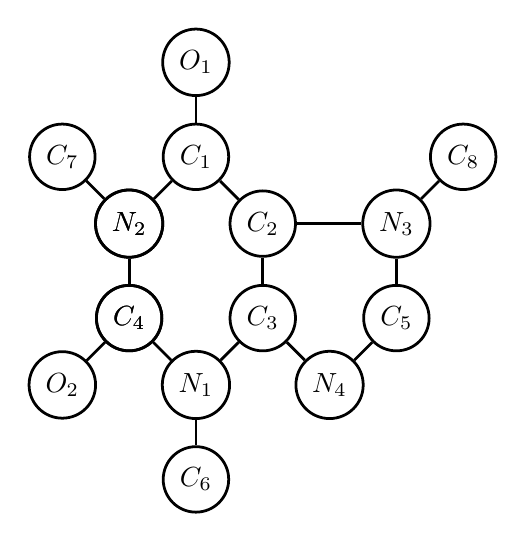
\begin{tikzpicture}[node distance={12mm}, line width=1pt, main/.style = {draw, circle}] 
\node[main] (1) []{$C_1$}; 
\node[main] (2) [below right of=1]{$C_2$}; 
\node[main] (3) [below of=2]{$C_3$}; 
\node[main] (4) [below left of=3]{$N_1$}; 
\node[main] (5) [above left of=4]{$C_4$}; 
\node[main] (6) [above of=5]{$N_2$};
\node[main] (9) [below right of=3]{$N_4$}; 
\node[main] (8) [above right of=9]{$C_5$}; 
\node[main] (7) [above of=8]{$N_3$}; 
\node[main] (10) [above of=1]{$O_1$}; 
\node[main] (11) [above left of=4]{$C_4$}; 
\node[main] (12) [above of=5]{$N_2$}; 

\node[main] (13) [below of=4]{$C_6$};  

\node[main] (17) [below left of=5]{$O_2$};

\node[main] (18) [above left of=6]{$C_7$}; 

\node[main] (22) [above right of=7]{$C_8$}; 



\draw [] (1) -- (2); 
\draw [] (2) -- (3); 
\draw [] (3) -- (4); 
\draw [] (4) -- (5); 
\draw [] (5) -- (6); 
\draw [] (6) -- (1); 
\draw [] (2) -- (7); 
\draw [] (7) -- (8); 
\draw [] (8) -- (9); 
\draw [] (9) -- (3); 
\draw [] (1) -- (10); 

\draw [] (4) -- (13); 

\draw [] (5) -- (17); 

\draw [] (6) -- (18); 

\draw [] (7) -- (22); 
\end{tikzpicture}
% \end{center}
}}
		\quad
		\subfloat[][A Path Decomposition]{\resizebox{0.16\textwidth}{!}{% !TEX root = ../main.tex
% \begin{center}
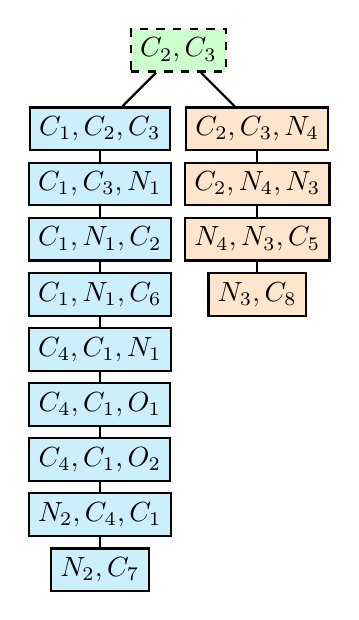
\begin{tikzpicture}[node distance={7mm}, thick, main/.style = {draw, rectangle}] 
\node[main, fill=green!20, dashed] at (0,0) (8) {$C_2,C_3$};
\node[main,fill=cyan!20] at (-1,-1) (7){$C_1,C_2,C_3$};
\node[main,fill=cyan!20] (100) [below of =7] {$C_1,C_3,N_1$};
\node[main,fill=cyan!20] (6) [below of =100]{$C_1,N_1,C_2$};
\node[main,fill=cyan!20] (5) [below of =6]{$C_1,N_1,C_6$};
\node[main,fill=cyan!20] (4) [below of =5]{$C_4,C_1,N_1$};
\node[main,fill=cyan!20] (3) [below of =4]{$C_4,C_1,O_1$};
\node[main,fill=cyan!20] (2) [below of =3]{$C_4,C_1,O_2$};
\node[main,fill=cyan!20] (1) [below of =2]{$N_2,C_4,C_1$};
\node[main,fill=cyan!20] (0) [below of =1] {$N_2,C_7$}; 

%\node[main,white] (00) [right = 1cm of 0] {}; 
%\node[main,white] (000) [left = 1cm of 0] {}; 



\node[main,fill=orange!20] at (1, -1) (9){$C_2,C_3,N_4$};
\node[main,fill=orange!20] (10) [below of =9]{$C_2,N_4,N_3$};
\node[main,fill=orange!20] (11) [below of =10]{$N_4,N_3,C_5$};
\node[main,fill=orange!20] (12) [below of =11]{$N_3, C_8$};


\draw [] (0) -- (1); 
\draw [] (1) -- (2); 
\draw [] (2) -- (3); 
\draw [] (3) -- (4); 
\draw [] (4) -- (5); 
\draw [] (5) -- (6); 
\draw [] (6) -- (100); 
\draw [] (7) -- (100); 
\draw [] (7) -- (8); 
\draw [] (8) -- (9); 
\draw [] (9) -- (10); 
\draw [] (10) -- (11); 
\draw [] (11) -- (12); 


\end{tikzpicture}
% \end{center}}}
		\quad
		\subfloat[][A Tree Decomposition]{\resizebox{0.3\textwidth}{!}{% \begin{center}
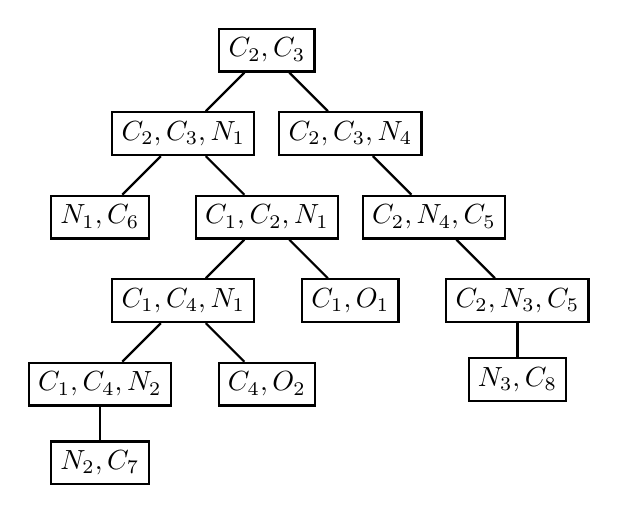
\begin{tikzpicture}[node distance={15mm}, thick, main/.style = {draw, rectangle}] 
\node[main] (0) []{$C_2,C_3$}; 
\node[main] (00) [below left of =0]{$C_2,C_3,N_1$};
\node[main] (000) [below left of =00]{$N_1,C_6$};
\node[main] (001) [below right of =00]{$C_1,C_2,N_1$};
\node[main] (0011) [below right of =001]{$C_1,O_1$};
\node[main] (0010) [below left of =001]{$C_1,C_4,N_1$};
\node[main] (00101) [below right of =0010]{$C_4,O_2$};
\node[main] (00100) [below left of =0010]{$C_1,C_4,N_2$};
\node[main] (001000) [below of =00100,,node distance={10mm}]{$N_2,C_7$};
\node[main] (01) [below right of =0]{$C_2,C_3,N_4$};
\node[main] (011) [below right of =01]{$C_2,N_4,C_5$};
\node[main] (0111) [below right of =011]{$C_2,N_3,C_5$};
\node[main] (01110) [below of =0111,,node distance={10mm}]{$N_3,C_8$};

\draw [] (0) -- (00); 
\draw [] (00) -- (000); 
\draw [] (00) -- (001); 
\draw [] (001) -- (0010); 
\draw [] (001) -- (0011); 
\draw [] (0010) -- (00100); 
\draw [] (00100) -- (001000);  
\draw [] (0010) -- (00101); 

\draw [] (0) -- (01); 
\draw [] (01) -- (011); 
\draw [] (011) -- (0111); 
\draw [] (0111) -- (01110); 

\end{tikzpicture}
% \end{center}}}
		\caption{A Graph Representation of Caffeine and a path and tree decomposition of this graph. Vertices in the root bag of the tree decomposition are highlighted in green (dashed). Notice how the removal of these nodes in the original molecule separates it into two connected components, each corresponding to one of the sides of the path decomposition, and one of the highlighted subtrees in the tree decomposition.}
		\label{fig:tree_dec_caffeine}
	\end{figure}

\end{example}
% \begin{figure}[H]
% 	\centerin{}g
% 	\chemfig{=^[:270](-[:330]=^[:30]-[:90]=^[:150]-[:210])-[:210]=_[:270](%
-[:330]=_[:30]-[:330]=_[:270]-[:210]=_[:150]-[:90])-[:210](-[:270]=_[:330]%
-[:270]=_[:210]-[:150]=_[:90]-[:30])=_[:150](-[:210]=_[:270]-[:210]=_[:150]%
-[:90]=_[:30]-[:330])-[:90](-[:150]=^[:90]-[:150]=^[:210]-[:270]=^[:330]%
-[:30])=_[:30](-[:330])-[:90]=^[:30]-[:90]=^[:150]-[:210]=^[:270](-[:330])}

% 	\caption{1,2,3,4,5,6-hexakis-phenylbenzene}
% 	\label{fig:tw_2 example}
% \end{figure}

\begin{lemma}[Proof in~\ref{app:proof}]\label{intseplemma}
	If $b$ is an introduce node with a single child $c$ and $X_b = X_c \cup \{v\}$, then $N(v)\cap G_b^\downarrow \subseteq X_c$. Here, $N(v)$ is the set of neighbors of $v.$
\end{lemma}



\begin{lemma}[Proof in~\ref{app:proof}]\label{joinseplemma}
	If $b$ is a join node with two children $c_1$ and $c_2,$ then in $G_b^\downarrow$ there is no edge with one endpoint in $V(G_{c_1}^\downarrow) \setminus X_b$ and the other in $V(G_{c_2}^\downarrow) \setminus X_b.$ Informally, $X_b$ is a cut that separates $V(G_{c_1}^\downarrow)$ from $V(G_{c_2}^\downarrow)$ in $G.$ See Figure~\ref{fig:tree_dec_caffeine}.
\end{lemma}

% \begin{proof}
% Let $T^\prime, T^{\prime\prime}, T^{\prime\prime\prime}$ be the subtrees of $T$ rooted at $b, c_1, c_2$ respectively. Let 
% $\mathcal{T}^\prime, \mathcal{T}^{\prime\prime}, \mathcal{T}^{\prime\prime\prime}$ be the corresponding tree decompositions. We will prove the given statement by contradiction. Therefore, let us assume that $u \in V(G_{c_1}^\downarrow) \setminus X_b$, $v \in V(G_{c_2}^\downarrow) \setminus X_b$, and $uv \in E(G_b^\downarrow)$.

% As $\mathcal{T}^{\prime}$ is a tree decomposition of $G^\downarrow_b$, there exists at least one bag $X_t$, such that $t \in \mathcal{T}^{\prime}$ and $u,v \in X_t$. From our initial assumption, we know that $u, v \notin X_b$, this implies that $t \neq b$. Therefore, either $t \in T^{\prime\prime}$ or $t \in T^{\prime\prime\prime}$. Without loss of generality, let us assume that $t \in T^{\prime\prime}$. As $v \in V(G_{c_2}^\downarrow) \setminus X_b$, there exists at least one bag $X_s$ such that, $ s \in T^{\prime\prime\prime}$ and $v \in X_s$. Observe that $v$ appears in both bags $X_s$ and $X_t$. Now by Definition \ref{def:tree_dec}, we know that $T^\prime_{v}$ is a connected subtree and any path connecting $s$ and $t$ goes through $b$. This implies that $X_b \in T^\prime_v$ and $v \in X_b$. This contradicts our initial assumption that $v \notin X_b$, hence completes the proof.
% \end{proof}
\section{Method}
\label{sec:method}

% \ml{``Inconsistent'' to ``large variation''}

% In this section, we propose our methods based on the observations in Section \ref{sec:motivation}.
In this section, we propose two techniques to further enhance the strong baseline to capture the variation of activation distributions better.
We first introduce spatial re-scaling to adapt the network to pixel-to-pixel variation.
We then propose channel-wise shifting and re-scaling to better capture the channel-to-channel variation.
Meanwhile, as both of the two methods are image-dependent, the image-to-image variation can be captured naturally.
By combining the two methods with our strong baseline, we build our enhanced BNN for SR, named EBSR.

% Because the activation distributions among pixels, channels and images have large variations \red{**are highly inconsistent} in SR networks, we introduce spatial re-scaling to adapt to pixel-wise variations and channel shift and re-scaling to adapt to channel-wise variations. And both of them are image-dependent to adapt to image-wise variations, which means during inference our network re-scales and shifts the distributions of activations flexibly for different input images. Based on these methods, we build an enhanced binary neural network for image super-resolution (EBSR).

% According to [3], the difference of activation magnitudes indicates different scaling factors are needed for each pixel.

\subsection{Spatial Re-scaling}
% It is better to use different scaling factors for different pixels to reduce the quantization error and retain more detailed information for image super-resolution. 

% \ml{In the main method, we do not need to introduce the previous works but can focus on introducing our own method. Channel rescaling in Real-to-binary Net is not relevant in this context.}

% Re-scaling the output of binary convolutions was proposed at the birth of BNN in XNOR-Net \cite{rastegari2016xnor} to reduce quantization error and improve accuracy for image classification tasks.
% It is computed as below:
% \begin{equation}
% \mathcal{A} * \mathcal{W} \approx(\operatorname{sign}(\mathcal{A}) \circledast \operatorname{sign}(\mathcal{W})) \odot \mathcal{K} \alpha
% \label{eq:xnor-net rescale}
% \end{equation}
% where $\circledast$ denotes the binary convolution and $\odot$ denotes the element-wise multiplication.
% $\mathcal{A}$, $\mathcal{W}$, $\alpha$, and $\mathcal{K}$ denote the activation, weight, weight scaling factor, and activation scaling factor, respectively.
%  Later in XNOR-Net++ \cite{bulat2019xnor}, Bulat et al. fuse the activation and weight scaling factors into a single one that is learned end-to-end based on gradients and this improves the classification accuracy on ImageNet dataset.

% % It is computed as Eq.~\ref{eq:xnor-net rescale}, where $\circledast$ denotes 
% %  the binary convolution and $\odot$ denotes the element-wise multiplication. The binary convolution of $\mathcal{A}$ and $\mathcal{W}$ is rescaled by the weight scaling factor $\alpha$ and the activation scaling factor $\mathcal{K}$, both of which are calculated analytically.


% \zc{Similarly, you should explain the meaning of A, W and the operators $\circledast$ in the formula}
% Then in Real-to-binary Net \cite{martinez2020training}, Martinez et al. used a data-driven channel re-scaling module that takes the pre-convolution activations as input to predict the activation scaling factor. Unlike that in XNOR-Net++ \cite{bulat2019xnor}, these scaling factors are not fixed during inference but rather inferred from data. By doing this, they further improved the classification accuracy on ImageNet over XNOR-Net++. 
As is shown in Figure \ref{fig:pixel}, activation distributions have large pixel-to-pixel variation in SR networks
and the difference of activation magnitudes indicates different scaling factors are preferred for different pixels.
Inspired by \cite{martinez2020training}, we propose spatial re-scaling to better adapt the network to the spatial variation
of activation distributions in SR networks.
% fit the various pixel-wise distributions in SR networks.
We take the real-valued activations $A$ before convolution as input and predict pixel-wise scaling factors $S(A)$, which re-scale the binary convolution output. Spatial re-scaling process can be formulated as follows:
\begin{equation}
A * W \approx(\operatorname{sign}(A) \circledast \operatorname{sign}(W)) \odot \alpha \odot S(A)
\label{eq:spatial rescale}
\end{equation}
where $\circledast$ denotes 
the binary convolution and $\odot$ denotes the element-wise multiplication. $A$, $W$, $\alpha$, and $S\left(A\right)$ denote real-valued activations, weights, the scaling factor of weights, and the spatial-wise scaling factor of activations respectively. $S\left(A\right) \in \mathbb{R}^{1\times H\times W}$ can be calculated with a convolution and a sigmoid function.
% as $\sigma\left( CONV\left(A\right)\right)$. 
As shown in Figure \ref{fig:method}(a), real-valued activations first go through a convolution layer,
which has an input channel of $C$ and an output channel of 1, 
and then pass through a sigmoid function to produce the scaling factors $S(A)$ along the spatial dimension.
During inference, the scaling factor will change dynamically according to different input feature maps.
By re-scaling binary convolution output using $S(A)$, we can reduce the quantization error and the original pixel-wise information in FP activation
will be preserved much better.
Spatial re-scaling leads to a large PSNR improvement of 0.24 dB (from 30.30 dB to 31.54 dB) on Set5 and 0.22 dB (from 25.09 dB to 25.31 dB)
on Urban100 compared with our strong baseline. 

\subsection{Channel-wise Shifting and Re-scaling}

\begin{table}[!tb]
\centering
\caption{Comparison between whether to fuse channel-wise shifting and re-scaling or not based on our baseline with spatial re-scaling. }
\label{tab:fusing}

\scalebox{0.65}{
\begin{tabular}{c|cc|cc|cc}
\hline
\multirow{2}{*}{Method}     & \multirow{2}{*}{OPs} & \multirow{2}{*}{Params} & \multicolumn{2}{c|}{Set5} & \multicolumn{2}{c}{Urban100} \\ \cline{4-7} 
                            &                      &                         & PSNR        & SSIM        & PSNR          & SSIM         \\ \hline
Baseline + spatial re-scale & 2.16G                & 0.05M                   & 31.54       & 0.883       & 25.31         & 0.759        \\
+ channel-wise shift and re-scale             & 2.34G                & 0.09M                   & 31.61       & 0.885       & 25.35         & 0.761        \\
+ w/ fusing                   & 2.27G                & 0.08M                   & \textbf{31.64}       & \textbf{0.885}       & \textbf{25.36}         & \textbf{0.761}        \\ \hline
\end{tabular}
}
\end{table}

In SR networks, activation distributions exhibit larger channel-to-channel variation (Figure \ref{fig:chl}).
Both the mean and magnitude of the activation distributions vary significantly across channels.
% Thus we use channel-wise shifting and re-scaling to adapt to various channel-wise distributions. 
\cite{martinez2020training} has proposed the data-driven channel re-scaling, 
but our method differs from them in further introducing data-driven thresholds to handle the channel-wise variation of both mean and magnitude.
Since the blocks to generate the scaling factors and thresholds are very similar, we further propose to fuse them into one module.
% and fusing channel-wise shifting and re-scaling into one module.
We evaluate the effect of fusing the two blocks in Table \ref{tab:fusing}.
With channel-wise shifting and re-scaling fused, our models have fewer operations and parameters overhead and slightly higher performance.

For the specific process, we take the real-valued activations as input and predict different thresholds and scaling factors for each channel. They are also image dependent, e.g., $\beta_{i}$ in Eq.\ref{eq:act_binarize} is no longer fixed during inference but generated according to different input feature maps. Channel-wise shifting and re-scaling can be formulated as follows:
\begin{equation}
A * W \approx(\operatorname{sign}(A-C_s(A)) \circledast \operatorname{sign}(W)) \odot \alpha \odot C_r(A)
\label{eq:channel-wise_shift_and_rescale}
\end{equation}
where $\circledast$ denotes 
the binary convolution and $\odot$ denotes the element-wise multiplication. $C_s(A), C_r(A) \in \mathbb{R}^{C\times1\times1}$ denote the channel-wise threshold and scaling factor, respectively. 
We show the block diagram in Figure \ref{fig:method}(b).
The real-valued input feature map is first squeezed to a ${C\times1\times1}$ vector by a global average pooling (GAP) layer.
The subsequent fully connected layers and ReLU learn the channel-wise information and output a ${2C\times1\times1}$ vector.
Then the ${2C\times1\times1}$ vector is split into two ${C\times1\times1}$ vectors.
We use the first $C$ channels as the channel-wise bias and pass the last $C$ channels through a sigmoid layer 
as the channel-wise scaling factor, which are used to shift the real-valued activations and re-scale the binary convolution output, respectively. 


% \ml{We can mention previously, channel-wise re-scale has been proposed. We propose to fuse them. Add the comparison between fuse v.s. no fuse.}

\begin{figure}[!tbp]%
  \centering
    \includegraphics[width=0.4\textwidth]{fig/methods.png}
  
% \subfloat[channel-wise shifting\&re-scale]{
%     \label{subfig:channel-wise shifting and re-scale}
%     \includegraphics[width=0.2\textwidth]{fig/chl shift and rescale.png}
%   }

  \caption{Block diagram for spatial re-scaling, and channel-wise shifting and re-scaling.} 
  % Input A is the real-valued activation tensor and C, H, and W denote its dimension. GAP stands for global average pooling. The reduction ratio r is set to 16 for a better trade-off between the performance and the number of operations and parameters.}
  \label{fig:method}
\end{figure}


\subsection{Network Structure}

Combining the spatial re-scaling and the channel-wise shifting and re-scaling methods, we construct the enhanced convolution layer (E-Conv).
Then we build our EBSR model based on E-Conv.
In Figure \ref{fig:E-conv}, we compare the binary convolution layer used in the baseline network and our proposed E-Conv.
We use spatial and channel-wise scaling factors to re-scale the binary convolution output,
and use channel-wise shifting to learn appropriate thresholds for each channel before binarization.
The scaling factors and threshold used in E-Conv are learnable and depend on the real-valued input activations.
In this way, our proposed EBSR can adapt to pixel-to-pixel, channel-to-channel, and image-to-image variations
to reduce the large binarization error and preserve more details.
% In this way, our proposed E-Conv reduces the large quantization error caused by binarization and keeps the original information of input feature maps to a large extent.


\begin{figure}[!tb]%
  \centering

    \includegraphics[width=0.5\textwidth]{fig/E-conv.png}

  \caption{Comparison of (a) the binary convolution layer with a skip connection used in our baseline network and (b) the proposed E-Conv.}
  \label{fig:E-conv}
\end{figure}


Figure \ref{fig:network} shows the basic block based on the E-Conv and our EBSR composed of the basic blocks. Following existing works, the convolution layers in the head and tail modules are not binarized. We choose the lightweight EDSR which has 16 basic blocks and 64 channels, and EDSR which has 32 basic blocks and 256 channels as our backbones, which correspond to EBSR-light and EBSR, respectively.

\begin{figure}[!tb]%
  \centering
  {
    \includegraphics[width=0.35\textwidth]{fig/network.png}
  }
  
  \caption{The structure of our proposed EBSR.  Convolution layers in purple are real-valued vanilla 3x3 convolutions.}
  \label{fig:network}
\end{figure}
\section{Related work}
% There is extensive recent work on speeding up analytical queries due to the need for consistent execution times in the face of the explosive growth in the volume of available data.
% In this section, we divide existing work into two categories: maintaining data freshness in MVs (\Cref{sec:server_side}) and optimizations for minimizing ad-hoc query latency (\Cref{sec:client_side}).

% \subsection{Maintaining Data Freshness in MVs}
% \label{sec:server_side}
% There exists a variety of data warehousing applications aimed at supporting low-latency analytical queries on fresh data.
% In particular, these applications require efficiency in the propagation of newly ingested data into downstream MVs.
 
\mypara{Efficient MV Refresh}
Incremental view maintenance (IVM) aims to update MVs to reflect newly ingested data, taking advantage of already computed results to perform the update in a manner more efficient than computing from scratch (full refresh)
~\cite{ahmad2012dbtoaster,mcsherry2013differential,armbrust2013generalized,zeng2016iolap, palpanas2002incremental, griffin1995incremental, agiwal2021napa, braun2015analytics}. 
There is an abundance of work in IVM, including incremental updates on duplicate values~\cite{griffin1995incremental}, non-distributive aggregate functions~\cite{palpanas2002incremental}, higher-order views~\cite{ahmad2012dbtoaster}, and sliding windows~\cite{braun2015analytics}. 
More recent works also investigate the scalability aspect of IVM, proposing scale-independent updates~\cite{armbrust2013generalized} and sampled views~\cite{zeng2016iolap}. Since \system is applicable to arbitrary SQL statements, \system is orthogonal to and is fully compatible with existing IVM techniques.

\mypara{MV Refresh Scheduling}
There exist works on scheduling the refresh of a MV set focusing on resolving cyclic dependencies~\cite{folkert2005optimizing}, minimizing weighted average staleness~\cite{golab2009scheduling}, and prioritizing MVs with the highest speedups on predicted future queries~\cite{ahmed2020automated}.
\system's scheduling to speed up the end-to-end refresh of the MV set is not addressed in existing works.

\mypara{DAG Workflow Scheduling}
The execution of workloads consisting of individual jobs with acyclic dependencies is a well-studied topic~\cite{apacheoozie,sparkdag,marchal2018parallel,bathie2020revisiting,baruah2022ilp}; many of these techniques can be applied to MV refresh runs studied in this paper.
Existing workflow scheduling systems such as Apache Oozie~\cite{apacheoozie}, Apache Airflow~\cite{airflow}, and Spark DAG scheduler~\cite{sparkdag} automate the execution of user-defined workflows following a topological order.
There are recent works aimed at finding more optimal execution orders in terms of peak memory usage~\cite{marchal2018parallel, bathie2020revisiting} and execution time on parallel platforms~\cite{baruah2022ilp}.
While \system is designed for use with MV refresh runs/workloads, our technique on joint scheduling and optimization can be reasonably applied to general workloads as a possible future direction.

% \paragraph{Incremental MV indexing}
% Update-optimized indices such as the log-structured merge-trees (LSM)~\cite{o1996log} are used for indexing MVs due to frequent updates induced by data ingestion~\cite{gupta2016mesa,agiwal2021napa}.
% \system is orthogonal to indexing: \system is capable of efficiently performing MV refresh runs regardless of whether the individual MVs are indexed or not.

% \subsection{Ad-hoc Query Latency Reduction}
% \label{sec:client_side}

% The minimization of ad-hoc analytical query response times is a well-studied topic due to latency being negatively correlated with the productivity of a data analyst during a data analysis session~\cite{liu2014effects}.
% Sessions are commonly conducted within visualization systems that contain a variety of optimization techniques to ensure that query response times fall within a certain latency tolerance.

% \mypara{Data prefetching}
% Data is often loaded into memory on a by-need basis in visualization systems to minimize interference with user-issued query computations~\cite{mani2017effective,xin2021enhancing,galakatos2017revisiting, yan2020auto, battle2016dynamic, crotty2016case, jalaparti2018netco}. 
% Query-time data retrieval can be significantly expedited by anticipating the data usage of the user in future queries and pre-loading the data into memory during the downtime between user queries (`think time'). SMART~\cite{mani2017effective} prefetches data for modified versions of current user-issued queries with different filters and dimensions. A-WARE~\cite{crotty2016case} maintains a sample store constantly refined through ingesting data based on speculations of future plots.
% ForeCache~\cite{battle2016dynamic} uses an SVM to predict the user's current analysis phase and accordingly prefetches data tiles partitioned based on different numerical values. NetCo predicts future queries via log analysis, and solves an ILP formulation to prefetch data to maximize the number of SLO-meeting queries~\cite{jalaparti2018netco}.
% In the case of MV refresh workloads, `think time' is nonexistent as individual MVs are refreshed back-to-back, rendering data prefetching techniques non-applicable.

\mypara{Intermediate Data Caching}
Some existing data visualization systems cache user-defined variables to support the typical incremental construction of data visualizations~\cite{zgraggen2016progressive, eichmann2020idebench} during data analysis sessions~\cite{jupyter, rstudio, colab}. 
Recent work proposes a management scheme for these cached variables under a memory constraint that greedily keeps variables with the highest estimated time savings based on predicted future user behavior via neural networks~\cite{xin2021enhancing}.
While useful for data visualization, a greedy approach to memory management fails to achieve satisfactory results compared to \system.

\mypara{Intermediate Result Reuse}

There exist works on storing intermediate results from computations to speedup future computations~\cite{yang2018intermediate, dursun2017revisiting, nagel2013recycling, michiardi2019memory, galakatos2017revisiting}.
Studied topics include the identification of reuse opportunities by finding overlaps in computation graphs of successive jobs~\cite{yang2018intermediate, michiardi2019memory},
selective storage under a space constraint with heuristics such as reuse probability~\cite{dursun2017revisiting}, expected savings~\cite{yang2018intermediate}, and recompute-storage cost difference~\cite{nagel2013recycling},
and rewriting incoming jobs to take advantage of stored intermediates~\cite{galakatos2017revisiting}.
These works share similarity with \system in their selection of items to store under a memory constraint, however, \system's problem setting requires it to uniquely consider the joint (re)ordering of job executions along with the selection of items.

% work that considers both job execution (re)order as well as intermediate result caching with a bounded amount of memory. but notably lack the joint aspect of \system and cannot be used to achieve immediate speedup on an incoming MV refresh run if no intermediates are stored beforehand. 

\mypara{Incremental Query Processing} Incremental processing (IQP) is useful for cases where not all data required for a query is immediately available. Similar to online aggregation~\cite{hellerstein1997online}, initial results of a query are computed on a subset of required data and progressively refined as the rest of the required data arrives in a predictable pattern~\cite{tang2019intermittent,wangtempura}. Tang et al. propose a dynamic programming formulation to pick intermediate states to store in memory given a limited memory budget~\cite{tang2019intermittent}. Tempura rewrites the query plan for more efficient execution based on predicted data arrival patterns~\cite{wangtempura}. While similarities exist between the problem setting of IQP and \system, such as management of bounded memory, \system notably includes additional joint optimization for the order of MV updates.

% \paragraph{Sampling}
% Sampling has seen wide use in visualization systems for reducing the computation time of ad-hoc queries by computing an approximate result over a subset of data as exact results are not always required by the user~\cite{crotty2016case, mani2017effective, zgraggen2014panoramicdata, kraska2021northstar, galakatos2017revisiting, kandula2016quickr}. 
% Commonly studied topics in sampling for ad-hoc queries include complex query sampling~\cite{kandula2016quickr}, rare event aggregation~\cite{kraska2021northstar, galakatos2017revisiting}, and maintaining consistency between related sampled visualizations~\cite{zgraggen2014panoramicdata}.
% Sampling server-side at the MV level compromises the assumptions of downstream applications and is thus not considered in \system.

% \paragraph{Progressive visualization}
% The latency tolerance for time-consuming queries can be circumvented by presenting a partially-computed visualization to the user within the tolerance, which is then incrementally refined until it is fully accurate~\cite{rahman2017ve, zgraggen2016progressive, crotty2015vizdom, kraska2021northstar, kamat2017infiniviz}.
% Example plots which benefit from progressive visualization include bar charts~\cite{kamat2017infiniviz} and heatmaps~\cite{rahman2017ve}.
% Similar to sampling, study on this topic is orthogonal to \system as pushing out partially-updated MVs compromises downstream assumptions.
We present in section~\ref{ssec:faces} an application of PnP-HVAE on face images, using a pretrained state-of-the-art hierarchical VAE. 
Next, we study the application of our framework to natural images. To that end, we introduce  in section~\ref{ssec:patchVDVAE}  a patch hierachical VAE architecture, that is able to model natural images of different resolutions. In section~\ref{ssec:app_nat}, we provide deblurring, super-resolution and inpainting experiments to demonstrate the relevance of the proposed method.

Additional results are presented in Appendix~\ref{app:add}. All experiments can be reproduced using the code available at \url{https://github.com/jprost76/PnP-HVAE}.



\subsection{Face Image restoration (FFHQ)}\label{ssec:faces}
We first demonstrate the effectiveness of PnP-HVAE on highly structured data, by performing face image restoration.
Latent variable generative models can accurately model structured images such as face images \cite{karras2019style,vahdat2020nvae,child2021very,kingma2018glow}, and then be used to produce high quality restoration of such data. 
In our experiments, we use the VDVAE model of~\cite{child2021very}, pre-trained on the FFHQ dataset~\cite{karras2019style}, as our hierarchical VAE prior.
VDVAE has $L=66$ latent variable groups in its hierarchy and generates images at resolution $256\times256$.

We compare PnP-HVAE with the intermediate layer optimization algorithm (ILO)~\cite{daras2021intermediate} that is based on a different class of generative models than HVAE. ILO is a GAN inversion method which optimizes the image latent code along with the intermediate layer representation of a StyleGAN to generate an image consistent with a degraded observation.
We use the official implementation of ILO, along with a StyleGAN2 model~\cite{karras2020analyzing, stylegan2pytorch}, that was trained for 550k iterations on images of resolution $256\times256$ from FFHQ.  
As VDVAE and StyleGAN models are not trained on the same train-test split of FFHQ, we chose to evaluate the methods on a subset of 100 images from the CelebA dataset~\cite{liu2018large}. 
For super-resolution, the degradation model corresponds to the application of a gaussian low-pass filter followed by a $\times 4$ sub-sampling, and the addition of a gaussian white noise with $\sigma=3$.
For the deblurring, we considered motion blur and  gaussian kernels, both with a noise level $\sigma=8$. %

We provide quantitative comparisons in table~\ref{table:comp_ILO}, along with a visual comparison of the results in figure~\ref{fig:face_restoration}.
PnP-HVAE has the best  PSNR and SSIM results for all the considered restoration tasks, while ILO provides better results  for the perceptual distance.
By jointly optimizing the image and its latent variable, PnP-HVAE provides  results that are both realistic and consistent with the degraded observation.
On the other hand,  ILO  only optimizes on an extended latent space. This method generates  sharp and realistic images with better LPIPS scores,   
but the results lack  of consistency with respect to the observation, which explains the overall lower PSNR performance. 






\subsection{PatchVDVAE: a HVAE for natural images}\label{ssec:patchVDVAE}
Available generative models in the literature operate on images of  fixed resolutions and
are either restrained to datasets of limited diversity, or even to registered face images~\cite{kingma2018glow,child2021very, vahdat2020nvae, karras2019style}, or requiring additional class information~\cite{brock2018large, dhariwal2021diffusion, song2020score, luhman2022optimizing}.
Fitting an unconditional model on natural images appears to be a more difficult task, as their resolution can change, and their content is highly diverse.
The complexity of the problem can be reduced by learning a prior model on patches of reduced dimension. 
For image restoration problems, the patch model can be reused on images of higher dimensions~\cite{zoran2011learning,prost2021learning,altekruger2022patchnr}. When the model is a full CNN, the prior on the set of the  patches can  be computed efficiently by applying the network on the full image~\cite{prost2021learning}.

We thus introduce  patchVDVAE, a fully convolutional hierarchical VAE.
Contrary to existing HVAE models whose resolution is constrained by the constant tensor at the input of the top-down block, patchVDVAE can generate images of different resolutions by controlling the dimension of the input latent. 
This amounts to defining a prior on patches whose dimension corresponds to the receptive field of the VAE. A similar model is used for image denoising in~\cite{prakash2021interpretable}.

 
For PatchVDVAE architecture, we use the same bottom-up and top-down blocks as VDVAE~\cite{child2021very}, and replace the constant trainable input in the first top-down block by a latent variable, to make the model fully convolutional (details on the  architecture are given in Appendix~\ref{app:details}). 
The training dataset is composed of $128\times 128$ patches extracted from a combination of DIV2K~\cite{agustsson2017ntire} and Flickr2K~\cite{Lim_2017_CVPR_workshops} datasets.
We perform data augmentation by extracting  patches at $3$ resolutions: HR-images and $\times 2$ and $\times 4$ downscaled images. 
The model is trained for $7.10^5$ iterations with a batch size of $64$. Following the recommendation of~\cite{hazami2022efficient}, we use Adamax optimizer with an exponential moving average and gradient smoothing of the variance.
We set the decoder model to be a gaussian with diagonal covariance, as in~\cite{luhman2022optimizing}.
PatchVDVAE is fully convolutional and can generate images of dimension that are multiples of $64$ as illustrated by
figure~\ref{fig:vdvae}.

\newlength{\patchwidth}
\setlength{\patchwidth}{0.135\columnwidth}
\begin{figure}[!ht]
    \centering
    \begin{subfigure}[t]{.34\columnwidth}\hspace{0.1cm}
        \setlength{\tabcolsep}{0.02pt}
\renewcommand{\arraystretch}{0}
        \begin{tabular}{*{2}{p{1.03\patchwidth}}}
            \includegraphics[width=\patchwidth]{figures_arxiv/patchVDVAE/samples/generated/64x64/setup-5-image-0018.png} &
            \includegraphics[width=\patchwidth]{figures_arxiv/patchVDVAE/samples/generated/64x64/setup-5-image-0016.png} \\
            \includegraphics[width=\patchwidth]{figures_arxiv/patchVDVAE/samples/generated/64x64/setup-5-image-0008.png} &
            \includegraphics[width=\patchwidth]{figures_arxiv/patchVDVAE/samples/generated/64x64/setup-5-image-0019.png}   
        \end{tabular}
    \end{subfigure}\hspace{-0.15cm}
    \begin{subfigure}[t]{.64\columnwidth}
\begin{tabular}{cc}\vspace{-0.1cm}
\includegraphics[width=2\patchwidth]{figures_arxiv/patchVDVAE/samples/generated/256x256/setup-2-image-0009.png}&
        \includegraphics[width=2\patchwidth]{figures_arxiv/patchVDVAE/samples/generated/256x256/setup-2-image-0002.png}\end{tabular}

    \end{subfigure}
    \caption{\label{fig:vdvae} Left: $64\times64$ patches samples from our patchVDVAE model trained on patches from natural images.
    Right: PatchVDVAE is fully convolutional and it can generate images of higher resolution (here: $128\times128$).\vspace{-0.2cm}}
\end{figure}

\subsection{Natural images restoration}\label{ssec:app_nat}
We  evaluate PnP-HVAE on natural image restoration.
For each task, we report the average value of the PSNR, the SSIM, and the LPIPS metrics on $20$ images from the test set of the BSD dataset~\cite{MartinFTM01}.\\


\noindent
{\bf Image deblurring.}
In the experiments, we consider $2$ gaussian kernels and $2$ motion blur kernels from~\cite{levin2009understanding}, with $3$ different noise levels 
$\sigma \in \{2.55, 7.65, 12.75\}$.
As a baseline we consider  EPLL~\cite{zoran2011learning}, which learns a prior on image patches with a gaussian mixture model.
We also compare PnP-HVAE  with PnP-MMO and GS-PnP, $2$ competing convergent Plug-and-Play methods based on CNN denoisers.
PnP-MMO~\cite{pesquet2021learning} restricts the denoiser to be contraction in order to guarantee the convergence of the PnP forward-backard algorithm. GS-PnP~\cite{hurault2022gradient} considers a gradient step denoiser and reaches state-of-the-art performances of non converging methods~\cite{zhang2021plug}.
We set the temperature $\tau$  in our method as $0.95$, $0.8$ and $0.6$ for noise levels $2.55$, $7.65$ and $12.75$ respectively, and we let it run for a maximum of $50$ iterations. 
For the three compared methods we use the official implementations and pre-trained models provided by the respective authors. 
Details on the choice of hyperparameters for the concurrent methods are provided in the Appendix~\ref{app:details}
Figure~\ref{fig:deblurring_bsd} illustrates that our method provides correct deblurring results. 

According to table~\ref{tab:deb}, the performance of PnP-HVAE is between those of EPLL and GS-PnP and it outperforms PnP-MMO for large noise levels.\\

\begin{table}
\begin{center}\footnotesize
    \begin{tabular}{>{\centering}m{.3cm}*{5}{c}}
    $\sigma$ &Method & PSNR$\uparrow$ & SSIM$\uparrow$ & LPIPS$\downarrow$  \\ 
    \hline
    \multirow{4}{*}{\vcell{$2.55$}}
    & PnP-HVAE & $27.75$ & $0.79$ & $0.31$\\
    & GS-PNP \cite{hurault2022gradient} & $\mathbf{29.59}$ & $\mathbf{0.84}$ & $\mathbf{0.22}$\\
    & EPLL \cite{zoran2011learning} & $26.49$ & $0.71$ & $0.36$\\ 
    & PnP-MMO \cite{pesquet2021learning} & $\underbar{29.50}$ & $\underbar{0.83}$ & $\underbar{0.20}$ \\ \hline
    \multirow{4}{*}{\vcell{$7.65$}}
    & PnP-HVAE & $\underbar{26.36}$ & $\underbar{0.72}$ & $\underbar{0.40}$\\
    & GS-PNP \cite{hurault2022gradient} & $\mathbf{27.33}$ & $\mathbf{0.77}$ & $\mathbf{0.31}$\\
    & EPLL \cite{zoran2011learning} & $24.04$ & $0.66$ & $0.45$ \\ 
    & PnP-MMO \cite{pesquet2021learning} & $25.34$ & $0.69$ & $0.34$\\
    \hline
    \multirow{4}{*}{\vcell{$12.75$}}
    & PnP-HVAE & $\underbar{25.12}$ & $\mathbf{0.73}$ & $\underbar{0.47}$\\
    & GS-PNP \cite{hurault2022gradient} & $\mathbf{26.32}$ & $\mathbf{0.73}$ & $\mathbf{0.37}$\\
    & EPLL \cite{zoran2011learning} & $23.28$ & $0.61$ & $0.51$ \\ 
    & PnP-MMO \cite{pesquet2021learning} & $22.42$ & $0.53$& $0.54$ \\
    \hline
    &\vspace*{-.3cm}\\
            \multicolumn{2}{c}{Blur and motion kernels}& \multicolumn{3}{c}{
        \includegraphics*[scale=1]{figures_arxiv/kernels/4.png}\;\includegraphics*[scale=1]{figures_arxiv/kernels/7.png}\;\includegraphics*[scale=1]{figures_arxiv/kernels/9.png}\;\includegraphics*[scale=1]{figures_arxiv/kernels/11.png}} 
    \end{tabular}
        \caption{\label{tab:deb}Comparison  of PnP-HVAE  and other restoration methods on deblurring. Results are averaged on $4$ kernels.\vspace{-0.2cm}}% on image deblurring.}
    \end{center}
\end{table}

\begin{figure}
    
    \begin{subfigure}[h]{\linewidth}
        \centering
        \includegraphics*[width=\columnwidth]{figures_arxiv/deb_s255_k7.pdf}\vspace{-0.1cm}
        \caption{Gaussian blur, $\sigma=2.55$}
    \end{subfigure}
    \begin{subfigure}[h]{\linewidth}
        \centering
        \includegraphics*[width=\columnwidth]{figures_arxiv/deb_s765_k11.pdf}\vspace{-0.1cm}
        \caption{Motion blur, $\sigma=7.65$}
    \end{subfigure}\vspace*{-0.1cm}
    \caption{\label{fig:deblurring_bsd} Natural image deblurring\vspace{-0.1cm}}
\end{figure}

\noindent {\bf Effect of the temperature.}
PnP-HVAE gives control on the temperature of the prior over the latent space.
In figure~\ref{fig:temp_effect}, we illustrate that reducing the temperature increases the strength of the regularization prior. In this example the tuning $\tau=0.7$ produces the best performance.\\
\begin{figure}[!ht]
   
    \includegraphics[width=\columnwidth]{figures_arxiv/demo_temp.pdf}\vspace{-0.15cm}
    \caption{ \label{fig:temp_effect} Effect of the temperature in PnP-VAE on a deblurring problem, with $\sigma=7.65$.\vspace{-0.15cm}}
\end{figure}


\noindent
{\bf Image inpainting.}
Next we consider the task of noisy image inpainting. 
We compose a test-set of 10 images from the validation set of BSD~\cite{MartinFTM01} and we create masks
  by occluding diverse objects of small size in the images. 
A gaussian white noise with $\sigma=3$ is added to the images.
As a comparaison, we still consider GS-PnP and EPLL.
For PnP-HVAE, the temperature is set to $\tau=0.6$, and the algorithm is run for a maximum of $200$ iterations, unless the residual $||\x_{k+1}-\x_k||$ is on a plateau.
We provide on Table~\ref{tab:inpainting_bsd} the distortion metrics with the ground truth, as well as a visual
\begin{table}



\begin{center}
    \begin{tabular}{cccc}
        & PSNR$\uparrow$ & SSIM$\uparrow$ &LPIPS$\downarrow$ \\\hline
        PnP-HVAE  & $\mathbf{29.54}$ & $\mathbf{0.93}$ & $\mathbf{0.06}$\\
        GS-PNP & $28.52$ & $\mathbf{0.93}$ & $0.09$\\
        EPLL & $\underline{29.16}$ & $\mathbf{0.93}$ & $\mathbf{0.06}$\\
    \end{tabular}
    \caption{\label{tab:inpainting_bsd}Quantitative evaluation for inpainting on BSD.}
    \end{center}
\end{table}
comparison on figure~\ref{fig:inpainting_bsd}. 
With its hierarchical structure,  PnP-HVAE outperforms the compared methods. \vspace{0.05cm}



\begin{figure}[!h]
    \includegraphics[width=\columnwidth]{figures_arxiv/demo_inp_bsd2.pdf}\vspace{-0.1cm}
    \caption{\label{fig:inpainting_bsd}Natural image inpainting\vspace{-0.3cm}}
\end{figure}











\section{Conclusion}\label{sec:conclusion}
In this work, we focus on addressing the fundamental challenge of OOD detection tasks, which is how to fully understand the semantic discrepancy between the ID/OOD samples. We reveal that the key to success in the realistic SCOOD task is to allocate as many ID samples in the unlabeled set correctly as possible. To this end, we propose a novel uncertainty-aware optimal transport scheme that introduces class-specific energy scores as guidance for effective label assignment. Experimental results show that our method achieves better performance than previous state-of-the-art methods on SCOOD benchmarks.

\textbf{Limitations.} In addition to temperature scaling, other techniques such as feature clipping applied in ReAct~\cite{sun2021react} also enhance the performance of energy score, so how to obtain an OOD score that best fits the SCOOD task can be further explored. Moreover, a setting highly related to SCOOD has been proposed in \cite{katz2022training} and formulated as a constrained optimization problem. We will also theoretically analyze these practical OOD settings in our feature work.

% \section*{Acknowledgments}
\textbf{Acknowledgments.} 
This work is supported by National Key R\&D Program of China under Grant 2020AAA0105701, National Natural Science Foundation of China (NSFC) under Grants 61872327, Major Special Science and Technology Project of Anhui, National Natural Science Foundation of China (62033012) and Ant Group through Ant Research Intern Program.

\section*{Acknowledgements}
This work was supported in part by the Institute of Information and communications Technology Planning and evaluation (IITP) grant funded by the Korea government (MSIT) (2021-0-00537), Benchmarks for UndeRstanding Grasping (BURG) (EP/S032487/1), National Natural Science Foundation of China under Grant No. 62073159 and Grant No. 62003155, Shenzhen Science and Technology Program under Grant No. JCYJ20200109141601708, and the Science, Technology and Innovation Commission of Shenzhen Municipality under grant no. ZDSYS20200811143601004.

\bibliography{bibliography.bib}
\bibliographystyle{unsrt}
\newpage
\appendix
\section{Appendix for Proofs}

\paragraph{Proof of Theorem \ref{thm:main}.}

\begin{proof}
\label{proof:main}
Our proof has two steps. In Step 1, we will show that SimCLR is equivalent to minimizing the cross entropy loss defined in Eqn.~(\ref{eqn:cross-entropy}). 
In Step 2, we will show  that minimizing the cross-entropy loss 
is equivalent to spectral clustering on $\bfpi$. 
Combining the two steps together, we have proved our theorem. 

\textbf{Step 1: } SimCLR is equivalent to minimizing the cross entropy loss.

The cross-entropy loss takes expectation over 
$\bfW_\bfX\sim \mathbb{P}(\cdot ; \bfpi)$, 
which means $\bfW_\bfX$ has exactly one non-zero entry in each row $i$. By Lemma~\ref{lem:multinomial}, we know every row $i$ of $\bfW_\bfX$ is independent of other rows. Moreover, 
$\bfW_{\bfX,i}\sim \mathcal{M}(1, \bfpi_i/\sum_j \bfpi_{i,j})=\mathcal{M}(1, \bfpi_i)$, because $\bfpi_i$ itself is a probability distribution.
Similarly, we know $\bfW_\bfZ$ also has the row-independent property by sampling over $\mathbb{P}(\cdot;\bfK_\bfZ)$.
Therefore, by Lemma~\ref{lem:cross_split}, we know Eqn.~(\ref{eqn:cross-entropy}) is equivalent to:
\[
 -\sum_{i=1}^n \mathbb{E}_{\bfW_{\bfX,i}}[\log \mathbb{P}(\bfW_{\bfZ,i}=\bfW_{\bfX,i};\bfK_\bfZ)],
\]

This expression takes expectation over $\bfW_{\bfX,i}$ for the given row $i$. Notice that 
$\bfW_{\bfX,i}$ has exactly one non-zero entry, which equals $1$ (same for $\bfW_{\bfZ,i}$). 
As a result
we expand the above expression to be:
\begin{equation}
 -\sum_{i=1}^n \sum_{j\neq i} \Pr(\bfW_{\bfX,i,j}=1)\log \Pr(\bfW_{\bfZ,i,j}=1).
\label{eqn:detailed-expansion}    
\end{equation}


By Lemma~\ref{lem:multinomial}, $\Pr(\bfW_{\bfZ,i,j}=1)=\bfK_{\bfZ,i,j}/\|\bfK_{\bfZ,i}\|_1$ for $j\neq i$. Recall that $\bfK_\bfZ=(k(\bfZ_i-\bfZ_j))_{(i,j)\in[n]^2}$, which means 
$\bfK_{\bfZ,i,j}/\|\bfK_{\bfZ,i}\|_1=\frac{\exp(-\|\bfZ_i-\bfZ_j\|^2/{2\tau})}{\sum_{k\neq i}
\exp(-\|\bfZ_i-\bfZ_k\|^2/{2\tau})
}$ for $j\neq i$, when $k$ is the Gaussian kernel with variance $\tau$. 

Notice that $\bfZ_i=f(\bfX_i)$, so we know
\begin{equation}
-\log \Pr(\bfW_{\bfZ,i,j}=1)=
-\log \frac{\exp(-\|f(\bfX_i)-f(\bfX_j)\|^2/{2\tau})}{\sum_{k\neq i}
\exp(-\|f(\bfX_i)-f(\bfX_k)\|^2/{2\tau}),
}
\label{eqn:infonce-equivalence}    
\end{equation}


The right hand side is exactly the InfoNCE loss defined in Eqn.~(\ref{eqn:infonce}).
Inserting Eqn.~(\ref{eqn:infonce-equivalence}) into Eqn.~(\ref{eqn:detailed-expansion}), we get the SimCLR algorithm, which first samples augmentation pairs $(i,j)$ with $\Pr(\bfW_{\bfX,i,j}=1)$ for each row $i$, and then optimize the InfoNCE loss. 

\textbf{Step 2: } minimizing the cross entropy loss 
is equivalent to spectral clustering on $\bfpi$.


By Lemma~\ref{lem:convert_to_spectral}, we may further convert the loss to 
\begin{equation}
\label{eqn:main-theorem-repul-attr}
\min_{\bfZ}
-\sum_{(i,j)\in [n]^2} \mathbf{P}_{i,j}
\log k (\bfZ_i-\bfZ_j)+\log \mathbf{R}(\bfZ).
\end{equation}
Since $k$ is the Gaussian kernel, this reduces to \[
\min_\bfZ \mathrm{tr}(\bfZ^\top \mathbf{L}(\bfpi) \bfZ)
+\log \mathbf{R}(\bfZ),
\]

where we use the fact that $\mathbb{E}_{\bfW_\bfX\sim \mathbb{P}(\cdot; \bfpi)}[\mathbf{L}(\bfW_\bfX)]
=\mathbf{L}(\bfpi)
$, because the Laplacian operator is linear and $
\mathbb{E}_{\bfW_\bfX\sim \mathbb{P}(\cdot; \bfpi)}(\bfW_\bfX)=\bfpi
$.
\end{proof}

\paragraph{Proof of Theorem \ref{thm:clip}.}
\begin{proof}
Since $\bfW_\bfX\sim \mathbb{P}(\cdot;\bfpi_{\mathbf{A}, \mathbf{B}})$, we know 
$\bfW_\bfX$ has exactly one non-zero entry in each row, denoting the pair that got sampled. 
A notable difference compared to the previous proof is we now have $n_\mathcal{A}+n_\mathcal{B}$ objects in our graph. CLIP deals with this by taking a mini-batch of size $2N$, 
such that $n_\mathcal{A}=n_\mathcal{B}=N$, and adding the $2N$ InfoNCE losses together. We label the objects in $\mathcal{A}$ as $[n_\mathcal{A}]$, and the objects in $\mathcal{B}$ as $\{n_\mathcal{A}+1, \cdots, n_\mathcal{A}+n_\mathcal{B}\}$. 

Notice that $\bfpi_{\mathbf{A}, \mathbf{B}}$ is a bipartite graph, so the edges of objects in $\mathcal{A}$ will only connect to object in $\mathcal{B}$ and vice versa. We can define the similarity matrix in $\cZ$ as $\bfK_\bfZ$, 
where $\bfK_\bfZ(i, j+n_\mathcal{A})=\bfK_\bfZ(j+n_\mathcal{A},i)= k(\bfZ_i-\bfZ_j)$ for $i\in [n_\mathcal{A}], j\in [n_\mathcal{B}]$, and otherwise we set $\bfK_\bfZ(i,j)=0$. 
The rest is same as the previous proof. 
\end{proof}

\paragraph{Proof of Theorem \ref{thm:exponential}.}

\begin{proof}
\label{proof:exponential}
Since the objective function consists of a linear term combined with an entropy regularization, which is a strongly concave function, the maximization problem is a convex optimization problem. Owing to the implicit constraints provided by the entropy function, the problem is equivalent to having only the equality constraint. We then introduce the Lagrangian multiplier $\lambda$ and obtain the following relaxed problem:

$$
\widetilde{E}(\boldsymbol{\alpha})=\psi_{1}-\sum_{i=1}^n \alpha_{i} \psi_{i}+\tau \sum_{i=1}^n \alpha_{i}\log \alpha_{i}+\lambda\left(\boldsymbol{\alpha}^{\top} \mathbf{1}_n-1\right).
$$

As the relaxed problem is unconstrained, taking the derivative with respect to $\alpha_{i}$ yields

$$
\frac{\partial \widetilde{E}(\boldsymbol{\alpha})}{\partial \alpha_{i}}=-\psi_{i}+\tau\left(\log \alpha_{i}+\alpha_{i} \frac{1}{\alpha_{i}}\right)+\lambda=0.
$$

Solving the above equation implies that $\alpha_{i}$ takes the form
$
\alpha_{i}=\exp \left(\frac{1}{\tau} \psi_{i}\right) \exp \left(\frac{-\lambda}{\tau}-1\right).
$ Since $\alpha_{i}$ lies on the probability simplex, the optimal $\alpha_{i}$ is explicitly given by
$
\alpha^{*}_{i}=\frac{\exp \left(\frac{1}{\tau} \psi_{i}\right)}{\sum_{i^{\prime}=1}^n \exp \left(\frac{1}{\tau} \psi_{i^{\prime}}\right)} .
$ Substituting the optimal point into the objective function, we obtain
$$
\begin{aligned}
E\left(\boldsymbol{\alpha}^*\right)  &=\psi_1-\sum_{i=1}^n \frac{\exp \left(\frac{1}{\tau} \psi_{i}\right)}{\sum_{i^{\prime}=1}^n \exp \left(\frac{1}{\tau} \psi_{i^{\prime}}\right)} \psi_{i}+\tau \sum_{i=1}^n \frac{\exp \left(\frac{1}{\tau} \psi_{i}\right)}{\sum_{i^{\prime}=1}^n \exp \left(\frac{1}{\tau} \psi_{i^{\prime}}\right)}\log \frac{\exp \left(\frac{1}{\tau} \psi_{i}\right)}{\sum_{i^{\prime}=1}^n \exp \left(\frac{1}{\tau} \psi_{i^{\prime}}\right)} \\
& =\psi_1 - \tau \log \left(\sum_{i=1}^n \exp \left(\frac{1}{\tau} \psi_{i}\right)\right).
\end{aligned}
$$
Thus, the Lagrangian dual function is given by
\begin{equation*}
-E\left(\boldsymbol{\alpha}^*\right)= -\tau \log \frac{\exp \left(\frac{1}{\tau} \psi_{1}\right)}{\sum_{i=1}^n \exp \left(\frac{1}{\tau} \psi_{i}\right)}.\qedhere
\end{equation*}
\end{proof}



\section{More on Experiments} \label{section: experiment_details}

\paragraph{CIFAR-10 and CIFAR-100} CIFAR-10 ~\citep{krizhevsky2009learning} and CIFAR-100 ~\citep{krizhevsky2009learning} are well-known classic image classification datasets. Both CIFAR-10 and CIFAR-100 contain a total of 60k $32 \times 32$ labeled images of different classes, with 50k for training and 10k for testing. CIFAR-10 is similar to CIFAR-100, except there are 10 different classes in CIFAR-10 and 100 classes in CIFAR-100.

\paragraph{TinyImageNet} TinyImageNet ~\citep{le2015tiny} is a subset of ImageNet ~\citep{deng2009imagenet}. There are 200 different object classes in TinyImageNet, with 500 training images, 50 validation images, and 50 test images for each class. All the images in TinyImageNet are colored and labeled with a size of $64 \times 64$.

\textbf{Pseudo-code.} Algorithm \ref{alg:Training Procedure} presents the pseudo-code for our empirical training procedure.

\begin{algorithm}[!htbp]
\caption{Training Procedure}
\label{alg:Training Procedure}
\begin{algorithmic}[1]
\REQUIRE trainable encoder network $f$, batch size $N$, augmentation strategy \textit{aug}, loss function $L$ with hyperparameters \textit{args}
\FOR {sampled minibatch ${x_i}_{i=1}^N$}
\FORALL{$i \in { 1, ..., N }$}
\STATE draw two augmentations $t_i = \textit{aug}\left(x_i\right) $, $t_i' = \textit{aug}\left(x_i\right) $
\STATE $z_i = f\left(t_i\right)$, $z_i' = f\left(t_i'\right)$
\ENDFOR
\STATE compute loss $\mathcal{L} = L(N, z, z', \textit{args})$
\STATE update encoder network $f$ to minimize $\mathcal{L}$
\ENDFOR
\STATE \textbf{Return} encoder network $f$
\end{algorithmic}
\end{algorithm}

We also provide the pseudo-code for our core loss function used in the training procedure in Algorithm \ref{alg:Core loss}. The pseudo-code is almost identical to SimCLR's loss function, with the exception of an extra parameter $\gamma$.

\begin{algorithm}[!htbp]
\caption{Core loss function $\mathcal{C}$}
\label{alg:Core loss}
\begin{algorithmic}[1]
\REQUIRE batch size $N$, two encoded minibatches $z_1, z_2$, $\gamma$, temperature $\tau$
\STATE $z = \textit{concat}\left(z_1, z_2\right)$
\FOR {$i \in {1, ..., 2N }, j \in {1, ..., 2N}$ }
\STATE $s_{i,j} = \Vert z_i - z_j \Vert_2^{\gamma}$
\ENDFOR
\STATE \textbf{define} $l(i, j)$ \textbf{as} $l(i, j) = - \log \frac{exp\left(s_{i,j}/\tau \right)}{\sum_{k=1}^{2N} \mathbf{1}{[k \ne i]} exp\left(s{i, j} / \tau \right)} $
\STATE \textbf{Return} $\frac{1}{2N} \sum_{k=1}^N\left[l(i, i+N) + l(i+N, i)\right]$
\end{algorithmic}
\end{algorithm}

Utilizing the core loss function $\mathcal{C}$, we can define all kernel loss functions used in our experiments in Table \ref{table: loss definition}. For all $z_i \in z$ with even dimensions $n$, we define $z_{L_i} = z_i\left[0:n/2\right]$ and $z_{R_i} = z_i\left[n/2:n\right]$.

\begin{table}[ht]
\centering
\begin{tabular}{{@{}l|l@{}}}
Kernel  &  Loss function \\ \midrule
Laplacian & $\mathcal{C}\left(N, z, z', \gamma=1, \tau\right)$\\ \midrule
Sum       & $\lambda * \mathcal{C}\left(N, z, z', \gamma=1, \tau_1\right) + (1-\lambda) * \mathcal{C}\left(N, z, z', \gamma=2, \tau_2\right)$  \\ \midrule
Concatenation Sum&$\lambda * \mathcal{C}\left(N, z_L, z'_L, \gamma=1, \tau_1\right) + (1-\lambda) * \mathcal{C}\left(N, z_R, z'_R, \gamma=2, \tau_2\right)$\\ \midrule
$\gamma = 0.5$ & $\mathcal{C}\left(N, z, z', \gamma=0.5, \tau\right)$          \\ 

\end{tabular}

\caption{Definition of kernel loss functions in our experiments}
\label {table: loss definition}
\end{table}

\textbf{Baselines.} We reproduce the SimCLR algorithm using PyTorch Lightning~\citep{PytorchLightning}.

\textbf{Encoder details.}
The encoder $f$ consists of a backbone network and a projection network. We employ ResNet50~\citep{ResNet} as the backbone and a 2-layer MLP (connected by a batch normalization~\citep{ioffe2015batch} layer and a ReLU \cite{nair2010rectified} layer) with hidden dimensions 2048 and output dimensions 128 (or 256 in the concatenation kernel case).

\textbf{Encoder hyperparameter tuning.}
For each encoder training case, we randomly sample 500 hyperparameter groups (sample details are shown in Table \ref{table: Hyperparameter sample}) and train these samples simultaneously using Ray Tune ~\citep{RayTune}, with the ASHA scheduler~\citep{li2018massively}. Ultimately, the hyperparameter group that maximizes the online validation accuracy (integrated in PyTorch Lightning) within 5000 validation steps is chosen for the given encoder training case.

\begin{table}[ht]
\centering

\begin{tabular}{@{}l|l|l@{}}
\midrule
Hyperparameter  & Sample Range & Sample Strategy \\ \midrule
start learning rate & $\left[10^{-2}, 10\right]$ & log uniform \\ \midrule
$\lambda$       & $\left[0, 1\right]$ & uniform \\ \midrule
$\tau$, $\tau_1$, $\tau_2$ & $\left[0, 1\right]$ & log uniform \\ \midrule
\end{tabular}

\caption{Hyperparameters sample strategy}
\label {table: Hyperparameter sample}
\end{table}

\textbf{Encoder training.} 
We train each encoder using the LARS optimizer~\citep{LARSOptimizer}, LambdaLR Scheduler in PyTorch, momentum 0.9, weight decay $10^{-6}$, batch size 256, and the aforementioned hyperparameters for 400 epochs on a single A-100 GPU.

\textbf{Image transformation.} The image transformation strategy, including augmentation, is identical to the default transformation strategy provided by PyTorch Lightning.

\textbf{Linear evaluation.}
The linear head is trained using the SGD optimizer with a cosine learning rate scheduler, batch size 64, and weight decay $10^{-6}$ for 100 epochs. The learning rate starts at $0.3$ and ends at $0$.

\textbf{Moco Experiments.} We also tested our method based on MoCo~\citep{he2019moco}. The results are summarized in Table \ref{tab:results-moco}. Here we choose ResNet18~\citep{ResNet} as the backbone and set a temperature of $0.1$ as default. For our simple sum kernel, we set $\lambda=0.8$. The results show that our method outperforms the original MoCo method.

\begin{table}[thb]
\centering
\caption{MoCo Experiment Results on CIFAR-10 and CIFAR-100.}
\label{tab:results-moco}
\resizebox{\textwidth}{!}{%
\begin{tabular}{@{}c|ccc|ccc@{}}
\toprule
\multirow{3}{*}{Method} & \multicolumn{3}{c|}{CIFAR-10} & \multicolumn{3}{c}{CIFAR-100} \\ \cmidrule(lr){2-4} \cmidrule(lr){5-7} 
                        & 200 epochs & 400 epochs    & 1000 epochs   & 200 epochs & 400 epochs & 1000 epochs         \\ \midrule
MoCo (repro.)         & $76.41 \pm 0.12$    & $80.01 \pm 0.15$          & $84.45 \pm 0.08$    & $\mathbf{47.02 \pm 0.11}$ & $52.50 \pm 0.07$ & $57.62 \pm 0.15$            \\
\midrule
Laplacian Kernel        & ${78.09 \pm 0.10}$    & $\mathbf{83.85 \pm 0.09}$          & $\mathbf{88.34 \pm 0.16}$    & $46.12 \pm 0.22$   & $53.44 \pm 0.17$ & $59.10 \pm 0.14$        \\
Simple Sum Kernel & $\mathbf{78.12 \pm 0.15}$   & $83.23 \pm 0.18$ & $87.50 \pm 0.20$ & $46.65 \pm 0.06$ & $\mathbf{53.62 \pm 0.19}$ & $\mathbf{59.83 \pm 0.12}$\\
\bottomrule
\end{tabular}
}
\end{table}



\section{More Experiments on Synthetic Data}


Consider a scenario with $n$ clusters, each containing $k$ vertices. Let the probability of vertices $u$ and $v$ from the same cluster belonging to $\bfpi$ be $p$. Conversely, for vertices $u$ and $v$ from different clusters, let the probability of belonging to $\pi$ be $q$. We generate the graph $\bfpi$ randomly, based on $p$ and $q$. We experiment with values of $k=100$ and $n=6$ for ease of visualization, embedding all points in a two-dimensional space. Each vertex's initial position originates from a normal distribution. In each iteration, we sample a subgraph of $\bfpi$ uniformly, ensuring each vertex has an out-degree of $1$. We then optimize the corresponding vectors using InfoNCE loss with an SGD optimizer and iterate until convergence. Our experimental setup consists of an SGD learning rate of $1$, an InfoNCE loss temperature of $0.5$, and a batch size of $50$. We evaluate two scenarios with different $p$ and $q$ values: $p=1$, $q=0$, and $p=0.75$, $q=0.2$. The results of these experiments are visualized in Figure \ref{fig:vis-spectral-cluster}. The obtained embeddings exhibit the hallmark pattern of spectral clustering of graph $\bfpi$.

\begin{figure}[!tb]
\centering
\subfigure{
\includegraphics[width=1\textwidth]{Figures/cluster_pi.png}
\label{fig:vis-cluster}
}
\subfigure{
\includegraphics[width=1\textwidth]{Figures/noised_cluster_pi.png}
\label{fig:vis-noised-cluster}
}
\caption{Visualizations of the optimization process using InfoNCE Loss on the vectors corresponding to $\bfpi$. Points of identical color belong to the same cluster within $\bfpi$. To showcase the internal structure of $\bfpi$, we randomly select 10 vertices from each cluster to display the edge distribution of $\bfpi$.}
\label{fig:vis-spectral-cluster}
\end{figure}



\end{document}